\documentclass[a4paper,fleqn,reqno,12pt,landscape]{article}

\usepackage{myarticlestyledefault}

\usepackage{lipsum}
\usepackage{vwcol}
\usepackage[]{paracol}
\usepackage[margin=1cm]{geometry}
\usepackage{pgfplots}

\setlength{\parindent}{0pt} % no indent globally

\newcommand{\mygray}[1]{\textcolor{gray}{#1}}
\newcommand{\mycomment}[1]{{\footnotesize \hfill \mygray{[#1]}}}
\newcommand{\myremark}[1]{{\footnotesize\mygray{#1}}}
\newcommand{\myrule}{\bigskip \hrule \bigskip \bigskip}

\date{}

\begin{document}

\thispagestyle{empty}

\noindent \textbf{A cheat sheet on measures from information theory (for the subjectively perplexed)} \hfill \textbf{Michael Franke}

\hrule

\bigskip

\columnratio{0.25}

\begin{paracol}{2}

  %%%%%%%%%%%%%%%%%%%%%%%%%%%%%%%%%%%%%%%%%%%%%%%%%%%
  % first column
  %%%%%%%%%%%%%%%%%%%%%%%%%%%%%%%%%%%%%%%%%%%%%%%%%%%

  \textbf{Notation}

  \medskip

  $X,Y$ are finite sets
  \\
  $P,P^{*} \in \Delta(X)$ \hfill \mycomment{$P,P^{*}$ distributions on $X$}
  \\
  $R \in \Delta(X \times Y)$ \mycomment{joint distribution}
  \\
  $P(x) = \sum_{y \in Y} R(x,y)$ \mycomment{marginal on $X$}
  \\
  $Q(y) = \sum_{x \in X} R(x,y)$ \mycomment{marginal on $Y$}

  \myrule

  \textbf{Info content (subjectivist version)}
  \medskip

  Info content $I_{P}(x)$ (``surprisal'') measures the perplexity of an agent with beliefs $P \in \Delta(X)$ when observing $x \in X$.
  \\
  \myremark{\hfill think of: neural activity in a predictive brain}

  \medskip

  \textbf{Definition}: $I_{P}(x) = - \log_{b} P(x)$
  \\
  \myremark{\hfill base $b>1$; common choice $b=2$ (bits)}

  \bigskip

  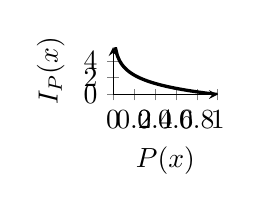
\begin{tikzpicture}
    \begin{axis}[
      width      = 0.24 \textwidth,
      height     = 0.18\textwidth,
      axis lines = left,
      xlabel = \(P(x)\),
      ylabel = {\(I_{P}(x)\)},
      ]
      % Below the red parabola is defined
      \addplot [
      domain=-0:1,
      samples=50,
      very thick,
      color=black,
      ]
      {-log2(x)};

      \addplot[
      mark=none,
      dotted,
      domain=-0:1,
      black,
      samples=2,
      ] {0};

    \end{axis}
  \end{tikzpicture}

  \medskip

  \textbf{Justification}: Negative log ($b>1$) is the only function satisfying constraints:

  \medskip

  {\myremark{if everything exactly as expected, zero perplexity}}
  \\
  If $P(x) = 1$, $I_{P}(x)=0$
  \medskip
  \\
  {\myremark{less expected, more perplexing}}
  \\
  If $P(x_{1}) > P(x_{2})$, then $I_{P}(x_{1}) < I_{P}(x_{2})$
  \medskip
  \\
  \myremark{perplexity adds up}
  \\
  $I_{P}(x_{1} \cap x_{2}) = I_{P}(x_{1}) + I_{P}(x_{2})$
  \\
  \myremark{ \hfill if $x_{1}, x_{2}$ stochastically independent}


  \switchcolumn

  %%%%%%%%%%%%%%%%%%%%%%%%%%%%%%%%%%%%%%%%%%%%%%%%%%%
  % second column
  %%%%%%%%%%%%%%%%%%%%%%%%%%%%%%%%%%%%%%%%%%%%%%%%%%%

  \hfill
  \begin{minipage}[t]{0.5\linewidth}
    \strut\vspace*{-\baselineskip}\newline
    \textbf{General template for all measures}

    \medskip

    Definitions below are all expected values of the form: \\
    \begin{minipage}[t]{0.3\linewidth}
      \strut\vspace*{-\baselineskip}\newline
      % \strut\vspace*{0.2cm} \hspace*{0.2cm}
      % \hfill $ \sum_{x \in X} P_{GT}(x) \ F(x) $ \hfill
      \begin{equation*}
        \sum_{x \in X} P_{GT}(x) \ F(x)
      \end{equation*}
    \end{minipage}
    \hspace*{-0.5cm}
    \begin{minipage}[t]{0.5\linewidth}
      \strut\vspace*{-\baselineskip}\newline
      \vspace*{-0.75cm}
      \begin{align*}
        & \text{\myremark{$P_{GT}$ is the assumed ground-truth}}\\
        & \text{\myremark{$F$ is some function related to perplexity}}
      \end{align*}
    \end{minipage}
  \end{minipage}
  \hfill
  \begin{minipage}[t]{0.23\linewidth}
    \strut\vspace*{-\baselineskip}\newline
    \textbf{Logarithm rules}

    \medskip

    % \myremark{inverse function of exponential}\\
    % \hspace*{0.1em }$x = a^{y} \ \  \Leftrightarrow  \ \  y = \log_{b} x$
    % \medskip
    % \\
    \myremark{change of base}\\
    \medskip
    $\log_{b} x = \frac{\log_{b} x}{\log_{b} b}$
  \end{minipage}
  \hfill
  \begin{minipage}[t]{0.2\linewidth}
    \strut\vspace*{-\baselineskip}\newline
    {\textcolor{white}{\textbf{Logarithm rules}}}

    \medskip

    % \myremark{product-to-sum rule}\\
    % \medskip
    % $\log_{b}( x y ) = \log_{b} x + \log_{b} y$
    % \\
    \myremark{division-to-subtraction rule}\\
    \medskip
    $\log_{b} \frac{x}{y} = \log_{b} x - \log_{b} y$
  \end{minipage}

  % \myrule

  \begin{center}
    \begin{tabular}[c]{lccccr}
      \toprule
      &
      & $\mathbf{P_{GT}}$
      & $\mathbf{F}$
      & \textbf{definition}
      \\ \midrule
      %%%%%%%%%%%%%%%%%%%%%%%%%%%%%%%%%%%%%%%%%%%%%%%%%%
      \textbf{entropy}
      & $\mathcal{H}(P)$
      & $P$
      & $I_{P}$
      & $- \sum_{x \in X} P(x) \ \log_{b} P(x) $ % & = - \sum_{x \in X} P(x) \ \log_{2} P(x)
      \\ \addlinespace[0.1em]
      %%%%%%%%%%%%%%%%%%%%%%%%%%%%%%%%%%%%%%%%%%%%%%%%%%
      \multicolumn{6}{l}{\myremark{average perplexity of an agent with beliefs $P$ when the ground truth is $P$}}
      \\ \addlinespace[1em]
      %%%%%%%%%%%%%%%%%%%%%%%%%%%%%%%%%%%%%%%%%%%%%%%%%%
      \textbf{cross-entropy}
      & $\mathcal{H}(P^*,P)$
      & $P^{*}$
      & $I_{P}$
      & $- \sum_{x \in X} P^{*}(x) \ \log_{b} P(x)$ % & = - \sum_{x \in X} P^{*}(x) \ \log_{2} P(x)
      \\ \addlinespace[0.1em]
      %%%%%%%%%%%%%%%%%%%%%%%%%%%%%%%%%%%%%%%%%%%%%%%%%%
      \multicolumn{6}{l}{\myremark{average perplexity of an agent with beliefs $P$ when the ground truth is $P^{*}$}}
      \\ \addlinespace[1em]
      %%%%%%%%%%%%%%%%%%%%%%%%%%%%%%%%%%%%%%%%%%%%%%%%%%
      \textbf{joint entropy}
      & $\mathcal{H}(P,Q)$
      & $R$
      & $I_{R'}$
      & $- \sum_{z \in X \times Y} R(z) \ \log_{b} R(z)$ % & = - \sum_{z \in X \times Y} R(z) \ \log_{2} R(z)
      \\ \addlinespace[0.1em]
      %%%%%%%%%%%%%%%%%%%%%%%%%%%%%%%%%%%%%%%%%%%%%%%%%%
      \multicolumn{6}{l}{\myremark{just entropy applied to a joint probability distribution; slightly boring but useful for the ``fun facts'' below}}
      \\ \addlinespace[-0.3em]
      \multicolumn{6}{l}{\myremark{NB: cross-entropy compares distributions on the same $X$, joint entropy looks at the joint distribution over product of space $X \times Y$}}
      \\ \addlinespace[1em]
      %%%%%%%%%%%%%%%%%%%%%%%%%%%%%%%%%%%%%%%%%%%%%%%%%%
      \textbf{conditional entropy}
      & $\mathcal{H}(P \mid Q)$
      & $Q$
      & $\mathcal{H}(R^{\mid y})$
      & $- \sum_{y \in Y} Q(y) \ \sum_{x \in X} R(x \mid y) \  \log_{b} R(x \mid y)$
      & \myremark{ \ \ where  $R^{\mid y}(x) = R(x \mid y)$}
      \\ \addlinespace[0.3em]
      %%%%%%%%%%%%%%%%%%%%%%%%%%%%%%%%%%%%%%%%%%%%%%%%%%
      &
      & $R$
      & $I_{S}$
      & $- \sum_{\tuple{x,y} \in X \times Y} R(x,y) \ \log_{b} R(x \mid y) $
      & \myremark{ \ \ where  $S(\tuple{x,y}) = R(x \mid y$)}
      \\ \addlinespace[0.1em]
      %%%%%%%%%%%%%%%%%%%%%%%%%%%%%%%%%%%%%%%%%%%%%%%%%%
      \multicolumn{6}{l}{\myremark{average entropy of an agent's conditional beliefs about $X$ after observing events from $Y$; how uncertain is the agent about $X$ when they observe $Y$}} \\ \addlinespace[-0.3em]
      \multicolumn{6}{l}{\myremark{two equivalent formulations here: the second is the usual (compact) definition; the first is easier to interpret}}
      \\ \addlinespace[1em]
      %%%%%%%%%%%%%%%%%%%%%%%%%%%%%%%%%%%%%%%%%%%%%%%%%%
      \textbf{relative entropy}
      & $D_{\text{KL}}(P \mid \mid Q)$
      & $P$
      & $I_{Q} - I_{P}$
      & $ \sum_{x \in X} P(x) \ \log_{b} \frac{P(x)}{Q(x)}$
      \\ \addlinespace[0.1em]
      %%%%%%%%%%%%%%%%%%%%%%%%%%%%%%%%%%%%%%%%%%%%%%%%%%
      \multicolumn{6}{l}{\myremark{also known as \textbf{Kullback-Leibler divergence}; average difference in perplexity when agent believes $Q$ instead of true $P$ }}
      \\ \addlinespace[-0.3em]
      \multicolumn{6}{l}{\myremark{``excess surprisal'' or ``unnecessary perplexity'' on top of the minimum (when having ``true beliefs'' $P$)}}
      \\ \addlinespace[1em]
      %%%%%%%%%%%%%%%%%%%%%%%%%%%%%%%%%%%%%%%%%%%%%%%%%%
      \textbf{mutual information}
      & $I(P, Q)$
      & $R$
      & $I_{R^{\Perp}} - I_{R}$
      & $ \sum_{\tuple{x,y} \in X \times Y} R(x,y) \ \log_{b} \frac{R(x,y)}{P(x)\ Q(x)}$
      & \myremark{\ \ where $R^{\Perp}(x,y) = P(x) \ Q(x)$}
      \\ \addlinespace[0.1em]
      %%%%%%%%%%%%%%%%%%%%%%%%%%%%%%%%%%%%%%%%%%%%%%%%%%
      \multicolumn{6}{l}{\myremark{excess perplexity of an agent believing that $X$ and $Y$ are independent, when in truth they might not be }} \\ \addlinespace[-0.3em]
      \multicolumn{6}{l}{\myremark{alternatively: how much learning about $Y$ reduces uncertainty about $X$ (and vice versa; see facts below)}} \\ \addlinespace[-0.3em]
      \multicolumn{6}{l}{\myremark{special case of KL-divergence for joint distributions, one treating $X$ and $Y$ as independent}} \\ \bottomrule
    \end{tabular}
  \end{center}


  \textbf{Fun facts}

  \begin{minipage}[t]{0.6\linewidth}
    \begin{multicols}{2}

      $P^{*} = \arg \min_{P}\mathcal{H}(P^{*}, P)$

      $\mathcal{H}(P,P) = \mathcal{H}(P) $

      $D_{KL}(P \mid \mid Q) = \mathcal{H}(P,Q) - \mathcal{H}(P)$

      $ \ $

      $I(P,Q) = I(Q,P)$

      $I(P,Q) = \mathcal{H}(P) - \mathcal{H}(P \mid Q)$

      $I(P,Q) = \mathcal{H}(P) + \mathcal{H}(Q) - \mathcal{H}(P,Q)$

      $ \ $

    \end{multicols}
  \end{minipage}
    \hfill
  \begin{minipage}[t]{0.35\linewidth}
    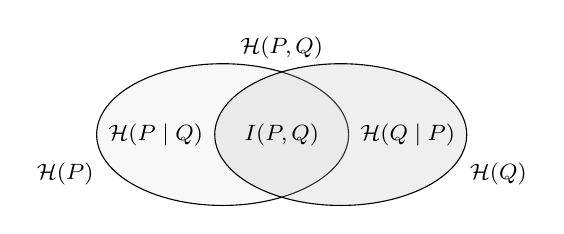
\begin{tikzpicture}
      \begin{scope}[shift={(3cm,-5cm)}, scale = 0.5]
        \draw[fill=gray!20, draw = black, fill opacity=0.25] (-1.5,0) ellipse (3.2 and 1.8);
        \draw[fill=gray!50, draw = black, fill opacity=0.25] (1.5,0)  ellipse (3.2 and 1.8);
        \node at (0,2.2)   (top)     {\footnotesize{$\mathcal{H}(P,Q)$}};
        \node at (-3.2,0)  (left)    {\footnotesize{$\mathcal{H}(P \mid Q)$}};
        \node at (3.2,0)   (right)   {\footnotesize{$\mathcal{H}(Q \mid P)$}};
        \node at (0,0)     (middle)  {\footnotesize{$I(P,Q)$}};
        \node at (-5.5,-1) (leftout) {\footnotesize{$\mathcal{H}(P)$}};
        \node at (5.5,-1)  (leftout) {\footnotesize{$\mathcal{H}(Q)$}};
      \end{scope}

    \end{tikzpicture}
  \end{minipage}
\end{paracol}

\end{document}
